\chapter{Knowledge Graphs}\label{chap:kgs}

\chapterQuote{\hfill\textit{``Knowledge is hot water on wool. It shrinks time and space.''}}{--- \textit{House of Leaves}, Mark Z. Danielewski}

\chapterAbstract{K}{nowledge Graphs (KGs) are ...}

% are collections of facts that are represented in a graph-like structure, with entities and connections between them. This chapter provides an introduction to KGs, and it is structured as follows: Section~\ref{sec:kgs-intro} introduces the reader to their history and main characteristics. Section~\ref{sec:kgs-current} provides an overview of the most prominent KGs in use nowadays. Section~\ref{sec:kgs-applications} presents some of the many practical applications of Knowledge Graphs. Section~\ref{sec:kgs-challenges} reflects on the main current challenges regarding KGs. At last, Section~\ref{sec:kgs-summary} summarizes and concludes this chapter.

\section{Introduction}\label{sec:kgs-intro}
% METER ESTA IDEA AQUI.
% Es gracioso que los grafos de conocimiento al fin y al cabo no representan nada "nuevo" ya que una base de datos relacional puede implementar grafos etc. Se puede mencionar la idea de que los grafos de conocimiento permiten quitar bagaje y tener algo simple de implementar, expandir, y al que aplicar algoritmos.

Before the emergence of knowledge graphs, information was predominantly stored in traditional databases and represented in tabular formats. While these databases were effective at storing structured data, they lacked the capacity to capture the complex relationships and semantics inherent in real-world information.

The concept of knowledge graphs can be traced back to the early days of Artificial Intelligence (AI) research. In the 1960s and 1970s, researchers began exploring methods to represent knowledge in a form that could be understood and utilized by computers. Early endeavors focused on semantic networks, which used nodes to represent concepts and edges to denote relationships between them.

The advent of the World Wide Web in the 1990s brought about an explosion of digital information. As the volume of web content grew, so did the need for more sophisticated methods of organizing and extracting knowledge from this vast repository. This led to the development of the Semantic Web, a vision championed by Sir Tim Berners-Lee, which aimed to make web content machine-understandable.

A pivotal milestone in the evolution of knowledge graphs was the introduction of the Resource Description Framework (RDF) in the late 1990s. RDF provided a standardized way to describe resources on the web and establish links between them. This laid the foundation for the creation of linked data, which allows for the interconnection of disparate datasets on the web.

In 2012, Google introduced the term "Knowledge Graph" as a central element of their search engine. Google's Knowledge Graph aimed to enhance search results by providing contextual information about entities and their relationships. This marked a significant shift towards a more semantically enriched approach to information retrieval.

Rather than a simple collection of relations between names of entities, they started to be seen as a rich, interconnected structure of elements (\textit{``things, not strings''}) with an enormous potential for practical and commercial applications. Many other large companies of the likes of Amazon, Facebook, Microsoft and eBay soon followed suit 
% \cite{shrivastava2017, krishnan2018, pittman2017, noy2019},
and the term Knowledge Graph (KG) rose to the popularity it still enjoys nowadays, replacing the denomination ``Knowledge Base''.

Today, knowledge graphs have become a cornerstone of various AI applications, including natural language processing, recommendation systems, and data integration. Their ability to represent complex relationships and semantic context has made them an invaluable tool in the era of big data and advanced machine learning techniques.

% kept this here for the citations...

% Representing and storing structured domain-specific knowledge has been an active research topic since at least 1970, when the first relational databases were introduced \cite{codd1970}. Given their indisputable success, many alternative means of representing knowledge in an structured manner have been proposed over the years. One of such proposals was using what was coined as a \textit{Knowledge Base} (KB) \cite{hayes-roth1983}, a collection of facts that are stored as direct relations between concepts. Contrary to relational databases, which need to go through a normalization process that introduces a number of indirections to represent a piece of knowledge, KBs were considered more straightforward to operate and reason about \cite{russell2020}. A number of Knowledge Bases were thus created and maintained throughout the subsequent years by multiple organizations and research entities, which were both general-purpose~\cite{mahdisoltani2014,lehmann2015dbpedia, rebele2016, carlson2010, bollacker2008, vrandevcic2014} and domain-specific~\cite{chakravarty2017, thorn2013pharmgkb, wishart2009, wishart2008, kanehisa2010}.

% The information inside a Knowledge Base was stored in the form of entities, which represented real-world or domain-specific concepts, and relations that link these entities together. This is known as a triple: a combination of two entities by means of a relation, which usually contains a verb. For example, a KB can represent the fact that Magnus Carlsen is a chess player using the triple \textit{(Magnus Carlsen, plays, Chess)}. Such triples were generally encoded in a KB using the RDF/XML format \cite{decker2000}, or an extension of it called RDFS, which allows for a higher degree of expressivity. However, since RDF/XML is mainly intended for machine use, later KBs also used other formats, like N3, Turtle, or RDF/JSON, which are more human-readable.

% However, the introduction of the Google Knowledge Graph in 2012 \cite{singhal2012} was a pivotal point for both the industrial use and academic research of Knowledge Bases.


% In the following sections, we present the most popular Knowledge Graphs that are under active use today and the ways in which they are constructed. We then discuss the many practical applications that can, and have been, derived from the usage of KGs in commercial and academical contexts. However, despite their many benefits, Knowledge Graphs still present several challenges that must be addressed to improve their functionality and usefulness. Therefore, we also provide an overview of the main open challenges that need to be addressed to refine and improve Knowledge Graphs.

\section{Modern Knowledge Graphs}\label{sec:kgs-current}

% Nowadays, there are a number of popular Knowledge Graphs under active use, either commercial or academical. Some of the most prominent ones are as follows:

\begin{itemize}
    \item \textbf{DBpedia} is a community-driven knowledge graph that extracts structured information from Wikipedia articles. It covers a wide range of topics and provides structured data about entities, their attributes, and relationships. DBpedia utilizes natural language processing and information extraction techniques to parse Wikipedia articles and convert unstructured text into a structured RDF format.
    
    \begin{figure}[!h]
        \centering
        \includegraphics[width=\textwidth]{fig/kgs/Keanu_DBpedia.png}
        \caption{The ontology \textit{Keanu Reeves} in DBpedia}
        \label{fig:kgs-dbpedia}
    \end{figure}
    
    \item \textbf{YAGO} (Yet Another Great Ontology) is a knowledge graph that combines data from Wikipedia, WordNet, and GeoNames. It provides a comprehensive representation of entities and their relationships. Created using automated extraction techniques and ontological alignment to integrate information from multiple sources.
    
    \item \textbf{Wikidata} is a collaborative, multilingual knowledge graph maintained by the Wikimedia Foundation. It serves as a central repository of structured data for Wikimedia projects and beyond, containing information about a diverse set of topics it is built by a global community of volunteers who contribute, edit, and curate data using a web-based user interface.
    
    \begin{figure}[!h]
        \centering
        \includegraphics[width=\textwidth]{fig/kgs/Keanu_Wikidata.png}
        \caption{The entity \textit{Keanu Reeves} in Wikidata}
        \label{fig:kgs-wikidata}
    \end{figure}

    % \item \textbf{GeoNames} is a geographical database that provides detailed information about places worldwide, including countries, cities, and landmarks. It also includes coordinates and population data, it combines data from various sources, including official government databases, with user contributions and validation processes.

    \item \textbf{UMLS (Unified Medical Language System)} is a comprehensive ontology and knowledge graph for the biomedical domain. It integrates terminology and data from various biomedical sources. UMLS is built through a combination of manual curation by domain experts and automated processes for integrating and mapping different terminologies.
    
    \item \textbf{Freebase (Now Part of Wikidata)} was a large-scale knowledge graph acquired by Google in 2010 and later integrated into Wikidata. It contained structured data on a wide array of topics, including people, places, and concepts. It was constructed through a combination of automated data extraction, crowd-sourcing, and expert curation.
    
    \item \textbf{WordNet} is a lexical database of the English language, organized in a semantic network. It groups English words into sets of synonyms (synsets) and provides short, general definitions. WordNet is manually constructed by lexicographers who define word meanings and establish semantic relationships between words.
    
    \item \textbf{NELL (Never-Ending Language Learning)} is a project aimed at creating a machine learning system that continuously learns to extract structured information from the web. It aims to discover new facts about entities over time it uses a combination of natural language processing, machine learning, and information extraction techniques to learn and update its knowledge base.
\end{itemize}

\section{Applications}\label{sec:kgs-applications}

Knowledge graphs, as we explored in the preceding chapter, are structured representations of information that emphasize the interconnectedness of entities, attributes, and relationships. This section delves into the practical applications and diverse utility of knowledge graphs across a spectrum of domains. The power of knowledge graphs lies not only in their capacity to organize information but in their ability to unlock a deeper layer of context, semantics, and relationships within data. 

They have emerged as a foundational tool in modern information processing and artificial intelligence. In this chapter, we delve into the diverse and powerful applications of knowledge graphs across various domains. From enhancing search engines to revolutionizing recommendation systems, knowledge graphs play a pivotal role in extracting valuable insights and enabling intelligent decision-making.

This chapter explores five prominent applications of knowledge graphs, each showcasing their versatility and impact in different realms of information processing, such as information retrieval, data analysis, and decision support. We illustrate how knowledge graphs have transformed traditional approaches, enabling more accurate, contextually aware, and personalized interactions with data.

\begin{itemize}
    \item \textbf{Semantic Search and Information Retrieval}:
    Knowledge Graphs provide a structured foundation for deducing the context between entities by understanding the intricate relationships between them. Unlike traditional keyword-based searches, semantic search engines, empowered by knowledge graphs, consider the deeper meaning and connections within the data, they ensure that search results are more accurate and contextually meaningful. This is especially crucial in fields like healthcare, legal research, and scientific studies where precision in information retrieval is essential. Through semantic search, users can navigate complex datasets with greater precision, uncovering insights that might be missed in traditional keyword-based searches.

    For instance, in a healthcare knowledge graph, the relationships between symptoms, diagnoses, and treatments allow for more precise and contextually relevant search results. This is vital in scenarios where accuracy and depth of information retrieval are paramount.

    
    \item \textbf{Recommendation Systems}:
    Knowledge graphs play a pivotal role in recommendation systems, revolutionizing how personalized suggestions are generated. 
    Recommendation systems, at their core, rely on understanding user behavior and preferences. Knowledge graphs provide the structured foundation needed to model these relationships effectively. By incorporating nuanced connections, recommendation systems can go beyond surface-level patterns, uncovering unexpected associations that lead to more meaningful and relevant suggestions.
    By modeling rich semantic connections between users, items, and their attributes, knowledge graphs enhance the accuracy and relevance of recommendations. 
    
    This is particularly crucial in domains like content streaming platforms, e-commerce, and content curation, where tailoring suggestions to individual tastes can significantly enhance the user experience. Knowledge Graphs elevate the accuracy and effectiveness of recommendation engines. This results in more engaged users, higher conversion rates, and ultimately, a more satisfying user experience.

    \todo{NLP and healthcare must be tweaked.}

    \item \textbf{Natural Language Processing (NLP)}:
    Knowledge graphs provide a structured framework for representing and understanding textual information. This allows for more accurate and nuanced language understanding, leading to improved tasks such as entity recognition, relationship extraction, and question answering. In a medical context, a knowledge graph can be used to understand clinical text. It can identify relationships between symptoms, diagnoses, and treatments, enabling the extraction of valuable information for healthcare applications.

    % second egneration here.

    Knowledge graphs provide a structured framework that significantly enhances natural language processing (NLP) tasks. They underpin advanced NLP functions such as entity recognition, relationship extraction, and question answering. By incorporating semantic relationships between entities and their attributes, knowledge graphs enrich language understanding. For example, in a medical knowledge graph, relationships can link symptoms, diagnoses, and treatments. This enables more precise and contextually relevant language comprehension in healthcare applications, where accuracy in understanding medical text is crucial.

    In the realm of language understanding, knowledge graphs serve as a fundamental tool for NLP applications. They allow for a more nuanced analysis of textual data by considering not just individual words, but also their relationships within a broader context. This is particularly valuable in fields like legal analysis, where the meaning of words and phrases depends heavily on the surrounding context. Knowledge graphs enable NLP systems to go beyond basic language processing, enabling them to grasp the complexities of human communication more effectively.

    Furthermore, knowledge graphs facilitate the inference of implicit relationships based on the existing graph structure. This means that even if a specific relationship is not explicitly stated in the text, the knowledge graph can help deduce it. This inference capability is a powerful feature in NLP tasks, enabling systems to uncover hidden patterns and connections within text data. This is particularly useful in tasks like sentiment analysis, where understanding the sentiment of a sentence may depend on the context provided by surrounding sentences.

    In conclusion, knowledge graphs are integral to natural language processing, providing a structured foundation that enhances tasks such as entity recognition, relationship extraction, and question answering. They allow for a more nuanced and accurate understanding of language by considering the contextual relationships between entities. This is crucial in fields where precision and context in language comprehension are paramount, such as healthcare, legal research, and sentiment analysis.

    \item \textbf{Contextual Analysis and Decision Support}:
    Contextual analysis involves examining information within the broader framework of its surroundings, considering the environment, relationships, and relevant circumstances that influence its meaning or interpretation. It is crucial in understanding the full significance of data. It helps in avoiding misinterpretations that can occur when information is considered in isolation. By taking into account the surrounding context, analysts can gain deeper insights and make more informed decisions. Knowledge graphs enhance contextual analysis by providing a structured framework for representing relationships and contextual information between entities. These graphs incorporate temporal, hierarchical, and semantic dimensions, allowing for a comprehensive understanding of data within its broader context. Moreover, knowledge graphs facilitate context-aware queries, enabling users to retrieve information based on specific contextual constraints. This not only supports decision-making but also empowers analysts to uncover hidden patterns and dependencies within the data, ultimately leading to more informed and effective analyses.

    \item \textbf{healthcare}:
    In healthcare, knowledge graphs serve as a powerful tool for representing, organizing, and analyzing complex medical information. They provide a structured framework that captures relationships between medical entities, their attributes, and contextual information. For instance, a healthcare knowledge graph can model the relationships between symptoms, diagnoses, treatments, medications, and patient histories. This enables comprehensive and contextually-rich representations of medical data, which is crucial for accurate diagnosis, treatment planning, and research.

    One of the key strengths of knowledge graphs in healthcare lies in their ability to integrate diverse sources of medical information. They can incorporate data from electronic health records (EHRs), medical literature, clinical trials, and other healthcare databases. This integration enables a holistic view of a patient's medical history and facilitates evidence-based decision-making by healthcare professionals.
    
    Furthermore, knowledge graphs support clinical decision support systems (CDSS) by providing a structured foundation for generating patient-specific recommendations and alerts. For example, a CDSS built on a healthcare knowledge graph can analyze a patient's symptoms, medical history, and medication interactions to offer tailored treatment suggestions. This not only enhances the quality of care but also helps healthcare providers stay up-to-date with the latest medical knowledge.
    
    In addition, knowledge graphs are invaluable for medical research and innovation. They enable researchers to explore relationships between genetic factors, diseases, treatments, and outcomes. This can lead to discoveries about disease mechanisms, personalized medicine approaches, and the development of new therapies.
    
    In summary, knowledge graphs play a vital role in healthcare by providing a structured framework for representing and analyzing medical information. They support accurate diagnosis, treatment planning, and research by capturing relationships between medical entities. Their ability to integrate diverse sources of medical data and support clinical decision-making makes them a fundamental tool in modern healthcare systems.

\end{itemize}

% \begin{itemize}
%     \item \textbf{Question answering:} Many search engines and personal assistants that are ubiquitous today, such as Siri, Alexa, Cortana, and Google Assistant, combine natural language processing (NLP) techniques, which helps them understand a query posed by a user, with Knowledge Graphs, which are used to navigate between entities and find the correct answer. Although most of the KGs that are used for this purpose are not made public for commercial reasons, they often contain a high amount of relations between both real-world and fictional entities and people. An example of this in practice is shown in Figure~\ref{fig:kgs-qa}.\\
    
%     \begin{figure}[!htp]
%         \centering
%         \includegraphics[width=\textwidth]{fig/kgs/qa.png}
%         \caption{Question answering using the Google Knowledge Graph}
%         \label{fig:kgs-qa}
%     \end{figure}

%     \item \textbf{Product recommendations:} Many authors \cite{zhang2021, palumbo2020, wang2019b, guo2022} have analyzed and proposed using Knowledge Graphs to issue product or media recommendations to users. By storing the relevant elements in a KG, such as the products that are on sale and the relations between them, and the users that bought or rated a product positively, one can apply a number of techniques to find a product that will be appealing to a new user in the system. The same concept can be applied for books or movies, a prime example of this is the movie information site IMDb, whose information has been used by Amazon to build a movie recommendation engine \cite{rele2022}.\newpage
    
%     \item \textbf{Advanced information retrieval:} Traditionally, information retrieval systems work by building and maintaining an index of a collection of documents and, when a user submits a query to the system, returns the documents that match the query more closely. However, this purely text-based approach falls short when it comes to semantical problems, for example, disambiguating an entity in the query, or interpreting it correctly. For this reason, some authors have proposed using Knowledge Graphs to enhance this process: for example, during the recent COVID-19 outbreak, \citet{wise2020} introduced a COVID-19 KG that aggregated the most recently published scientific works regarding this disease. This KG could be queried to quickly retrieve relevant research efforts, facilitating a worldwide collaboration to quell the pandemic.\\
    
%     \item \textbf{Education:} Multiple KG-centered proposals have been made in recent years to aid in several aspects of education. For example, \citet{chen2018} presented KnowEdu, a tool made for the purpose of building Knowledge Graphs out of educational materials. It is able to extract the main concepts of a subject or course, and then builds relations between them according to the activities and evaluation activities that the students will have to carry out in the future. \citet{aliyu2020} proposed building a KG containing the teachers, courses and scientific literature for a university, and using it to recommend relevant courses and books to students.\\
    
%     \item \textbf{Research:} Besides the previously discussed MAKG, a number of other Knowledge Graphs of research and academic entities have been built to help researchers explore possible lines of investigation and find possible relevant related materials. AceKG, introduced by \citet{wang2018}, is a similar KG, containing more than 3 billion triples with information about authors, papers, venues, and so on. The Artificial Intelligence KG \cite{dessi2020aikg}, and its extension, the Computer Science KG \cite{dessi2022cskg}, also contain a large volume of information pertaining research concepts, materials, tasks, and other similar entities in these fields. Furthermore, \citet{angioni2021} introduced the Academia/Industry KG, to help researchers identify trends in the constant exchanges between these two realms.\\
    
%     \item \textbf{Healthcare:} It is undoubtable that having an efficient and effective healthcare system is a cornerstone of a functional modern society. To help manage the ever-growing amount of medical data and records that healthcare professionals have to deal with, some proposals to integrate KGs in this field have been made. \citet{zhang2020b} presented HKGB, a KG builder aimed towards healthcare professionals that leverages their expertise to construct medical Knowledge Graphs. \citet{gong2021} proposed constructing KGs with information about medicines, diseases and patients, in order to use it to suggest medicines to patients with particular incompatibilities or intolerances.
% \end{itemize}

\section{Open challenges}\label{sec:kgs-challenges}
The original subsections for this section was:
\begin{itemize}
    \item Integration
    \item Correction
    \item Completion
\end{itemize}

a more relevant subset for this paper could be:

\begin{itemize}
    \item Integration - knowwing which entities represent the same thing.
    \item Completion - adding missing links which are implicit.
    \item Reasoning - explainability to the new knowledge found.
\end{itemize}

as all of them are relevant for the topic.

offer special interest to completion and reasoning as they are more interesting towards the work presented.

% Despite the fact that Knowledge Graphs are already a well-established concept in research and industry, a number of challenges about their use and refinement still remain \cite{paulheim2017, hogan2020, peng2023}. In the following subsections, we delve into some of the most prominent ones in more detail. 

% \subsection{Integration}
% It is common that more than one Knowledge Graph contain information about the same real-world concept or entity. While each individual KG may include different additional information complementing it, it would be desirable that said information be integrated together, so as to have a single source of truth that contains a more comprehensive set of facts. The process of joining two or more Knowledge Graphs together is known as KG integration or fusion.

% The most challenging step of this process is determining which entities in different KGs refer to the same one in the real world, a task known as entity alignment \cite{ren2022}. Although this has been a very active research topic, some future directions can still be further explored. For example, it is still not clear how this can be done reliably when the KGs to be integrated have different languages, which could be useful for multilingual recommendation systems or question answering \cite{javed2021}. An attempt in this regard has been made by \citet{xu2019} using neural networks, however, the alignment accuracy they obtain is still not high enough to perform this process reliably.

% Moreover, most KG fusion approaches assume that the Knowledge Graphs to be fused together are of the same modality. This falls short in the presence of multi-modal KGs, for example, the previously discussed FreeBase. Joining together two or more KGs which entities can be represented in different formats is still an open challenge, although some authors have made recent proposals. \citet{guo2021} have presented HMEA, a multi-modal entity alignment technique by using hyperbolic spaces. \citet{cheng2022} proposed MultiJAF, a framework for multi-modal entity alignment. Despite this, the wide array of possible modalities that could be represented through a KG make multi-modal alignment a very challenging and still unsolved task.

% Furthermore, a related problem is entity disambiguation. This problem presents itself during the process of building the KG, and consists in determining the specific meaning of an entity written in natural text in the presence of ambiguity. For example, contextual information is required to determine whether \textit{``Armstrong''} refers to the astronaut, the jazz musician, or the cyclist. If this is not solved correctly, even a successful entity alignment can be poisoned by the fact that the entities that were aligned were not disambiguated properly upon their creation, and thus do not actually refer to the same concepts.

% \subsection{Correction}
% The previous analysis of the most popular Knowledge Graphs shows that automatic construction is the most common way to build a KG, due to the sheer amount of facts that they are intended to contain. It is therefore inevitable that these automated methods introduce a certain degree of incorrect information in the KG, either because it was not correctly interpreted, or because the original source of information was wrong.

% Refining a KG after its creation by detecting wrong facts is known as Knowledge Graph correction. The most common way to perform this task is to do fact validation \cite{paulheim2017}, which assigns a confidence score in the interval $[0, 1]$ to every triple in the KG. Then, the triples that do not meet a minimum confidence threshold are purged from the graph.

% There exist a number of research works in the literature that propose different ways to do fact validation. \citet{pasternack2010} propose converting the facts in a KG into natural language sentences, and then using more general methods for fact checking. The same authors \cite{pasternack2011} also propose an alternative method, which groups up similar facts in a KG that provide support for each other, and then joins these groups to create more general justifications for the possible correctness of a fact. \citet{gerber2015} have proposed using classifiers, which can learn which facts are wrong by using a number of features. Of course, this requires that a manually-annotated set of correct and wrong triples is provided, which can be an arduous task. Another classification-based approach is proposed by \citet{syed2018}, in this case, based on textual evidence.

% A more refined ---and challenging--- approach to KG correction is to not only detect which facts are wrong, but to amend them if possible so that they represent correct knowledge. This is known as fact repairing. Due to the increased difficulty of the task, a smaller body of work can be found in the literature. \citet{topper2012} proposed leveraging the ontology of a Knowledge Graph to detect and fix inconsistencies in triples where the domain or range restrictions of the relation are violated, however, their proposal requires a human to step in and select the correct version of it out of the suggestions provided by the system. \citet{bonatti2011} proposed a fully-automated method for fixing triples, but it requires provenance and trust annotations to be present in the KG, which are relatively rare.

% \subsection{Completion}
% As previously discussed, most KGs are commonly built by extracting non-structured or semi-structured information from web sources, though some KGs can be manually curated by domain experts. When information extraction systems are applied to extract knowledge from online sources, that information is then semantized~\cite{ayala2018, neumaier2016} and stored in a KG as triples in the KG. Regardless of the specific process by which a KG is constructed, the resulting graph usually lacks a certain amount of information, either because said information was not originally present in the information source, or because it was unsuccessfully extracted or semantized~\cite{bordes2014b}. 

% Because of this inherent incompleteness, KGs operate under the Open World Assumption, i.e., a piece of information that is not present in a KG is not considered to be incorrect, but rather just unknown~\cite{galarraga2015}. Therefore, it is mandatory to refine KGs after their creation in order to expand the knowledge they contain~\cite{paulheim2017}.

% Deriving additional knowledge from an existing KG with the goal to augment it is a task known as Knowledge Graph completion~\cite{paulheim2017, shen2022overview}. In KG completion, the goal is to identify triples that are missing from the KG and have a chance of being correct that is as high as possible. To achieve this goal, a series of steps are usually carried out, which are visually depicted in Figure~\ref{fig:kgc-workflow}.

% \begin{figure}[!htp]
%     \centering
%     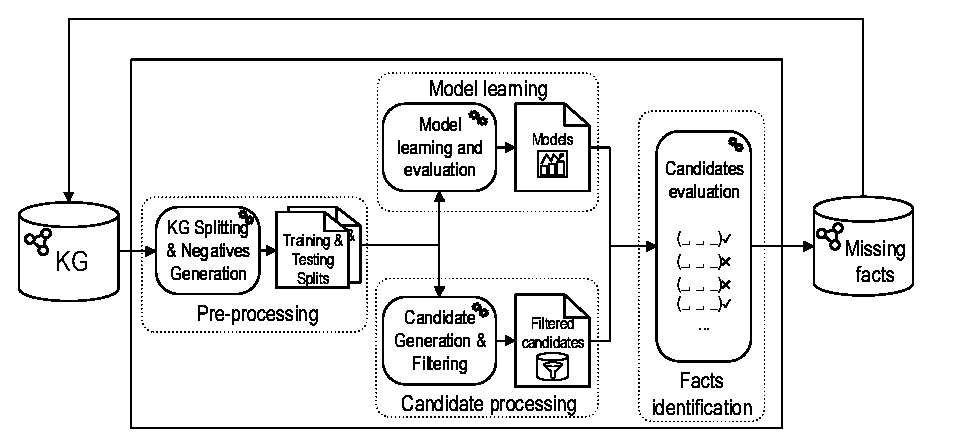
\includegraphics[width=\textwidth]{fig/kgs/kgc_workflow}
%     \caption{Knowledge Graph completion workflow}
%     \label{fig:kgc-workflow}
% \end{figure}

% First, the Knowledge Graph must be pre-processed in order to add negative triples, in the case they are not present, and split them between a training and a testing set \cite{ayala2019}. Then, a KG completion model is trained and evaluated using the sets of triples generated in the previous step. In parallel, a set of plausible candidate triples is materialized. If the KG completion model yields a satisfactory efficacy after its evaluation, it is applied on the candidate triples, to identify which ones are correct and which ones should be discarded \cite{borrego2021, borrego2019,shen2022overview}. Finally, the triples considered correct are added back to the Knowledge Graph, enriching it.

% In opposition to the previous two challenges, which focus on information that is already present in the graph, KG completion, by definition, focuses on finding knowledge that is not yet present. For this reason, it is particularly hard, and a number of authors have made different proposals to tackle it. Since the focus of this dissertation is on Knowledge Graph completion, the following chapters provide a more in-depth analysis of the existing proposals in the scientific literature to complete Knowledge Graphs.

\section{Summary}\label{sec:kgs-summary}
% This chapter has introduced the reader to Knowledge Graphs. It has provided a brief summary of their history and main characteristics, as well as a summary of the most prominent KGs that can be found today. Furthermore, it has presented the reader with an ample repertoire of practical applications of Knowledge Graphs, many of which we use in our daily lives. Finally, it has introduced some of the challenges regarding KGs that still remain open to this day, namely: Knowledge Graph integration, correction, and completion.

a brief summary of all topics in this chapter.
